\documentclass[12pt,parskip]{komatufte}
\usepackage[subpreambles=false]{standalone}

%%%%%%%%%%%%%%%%%%%%%%%%%%%
% Silence warning messages
\usepackage{silence}
\WarningsOff[scrlayer-notecolumn]
\WarningsOff[biblatex]

%%%%%%%%%%%%%%%%%%%%
% Commenting

%\usepackage[author=Lyndon]{pdfcomment}
%\newcommand{\pdfcomment}[1]{} %ignore all comments

%\usepackage{todonotes}
%\newcommand{\pdfcomment}{\todo}


%%%%%%%%%%%%%%%%%%%%
% Tables
\usepackage{booktabs}

%%%%%%%%%%%%%%%%%%%
% Fonts
\usepackage{tgadventor} %sans
\usepackage{tgpagella}  %serif
\usepackage{inconsolata} %mono
\usepackage[T1]{fontenc}

\usepackage{microtype}
\usepackage[all]{nowidow}
%%%%%%%%%%%%%%%%%%%%%%%
% Styling
\setcounter{secnumdepth}{4}
\setcounter{tocdepth}{2}

\usepackage{placeins}



%%%%%%%%%%%%%%%%%%%
% Math
\usepackage{amsmath, amssymb, stmaryrd, mathtools}
\DeclareMathOperator*{\argmin}{argmin}
\DeclareMathOperator*{\argmax}{argmax}

\usepackage{xparse,xstring,etoolbox}
% crossref this against notation section
\newcommand{\vv}[1]{\tilde{#1}} % vector
\newcommand{\seq}[1]{\mathcal{#1}} % sequence
\newcommand{\set}[1]{\mathbb{#1}} % set

%%%%%%%%%
% Indexing/sequence indexing
\newcommand{\seqind}[2]{#1^{#2}} % seqence index
\newcommand{\ind}[2]{#1_{#2}} % indexed
\newcommand{\disamb}[2]{#1^{\mathrm{#2}}} %disambiguated

%% Smart indexing and naming
\newcommand{\ifupper}[3]{
    \normalexpandarg
	\exploregroups
	\StrCount{ABCDEFGHIJKLMNOPQRSTUVWXYZ}{#1}[\uppercount]
	\ifnumgreater{\uppercount}{0}{#2}{#3}
}

%smart index
\DeclareDocumentCommand{\ii}{u{_} m}{
	\ifupper{#1}%
	{% just a single uppercase character, i.e. a matrix
		  %make sure the index is the right length
		\StrCount{#2}{,}[\indcount]
		\ifnumgreater{\indcount}{0}
		{ % Got multiple indexes so all good
		 	\ind{#1}{#2}
		}
		{ % Only 1 index so grab the column
		 	\ind{#1}{{:,#2}}
		}
	}%
	{% Not just a single upper case character
		\ind{#1}{#2}
	}
}

\DeclareDocumentCommand{\nn}{u{_} m}{
	\seqind{#1}{#2}
}

\DeclareDocumentCommand{\dd}{u{_} m}{
	\disamb{#1}{#2}
}

% Index of a vector
\DeclareDocumentCommand{\iv}{u{_} m}{\ii{\vv #1}_{#2}}
\DeclareDocumentCommand{\dv}{u{_} m}{\dd{\vv #1}_{#2}}
\DeclareDocumentCommand{\nv}{u{_} m}{\nn{\vv #1}_{#2}}

%exp
\let\oldexp\exp
\renewcommand{\exp}[1]{\oldexp \left( #1 \right)}
\newcommand{\exptwo}[1]{\oldexp_2 \left( #1 \right)}

\newcommand{\softmax}{\mathrm{smax}}

\DeclareMathOperator*{\expectedop}{\mathbb{E}}
\DeclareDocumentCommand{\expected}{u{_} m}{
	\expectedop\limits_{\mathrlap{#2}}
}

%%%%%%%%%%%%%%%%
%Graphics
\usepackage{tikz}
\usetikzlibrary{positioning, fit,  shapes.geometric}
\usepackage{ifthen}
\usepackage{etoolbox}

\tikzset{
	backgroundcolor/.style ={fill=white},
	every node/.append style={
		minimum height=7mm,
	},
	labe/.append style={
		%Blue,
		align = center,
		backgroundcolor,
		fill opacity=0.6,
		text opacity=1,
		font={\footnotesize\itshape}	
	},
	layer/.append style={
		draw,
		align = center,
		minimum height=7mm,
	},
	tight/.append style={
		inner sep=0.2mm,
	},
	lookupbox/.append style={
		draw=none,
		append after command={
		       	[shorten <= -0.5\pgflinewidth]
		       	([shift={(-1.5\pgflinewidth,-0.5\pgflinewidth)}]\tikzlastnode.north east)
		       	edge([shift={( 0.5\pgflinewidth,-0.5\pgflinewidth)}]\tikzlastnode.north west) 
		       	([shift={( 0.5\pgflinewidth,-0.5\pgflinewidth)}]\tikzlastnode.north west)
		       	edge([shift={( 0.5\pgflinewidth,-1.5\pgflinewidth)}]\tikzlastnode.south west)            
		       	([shift={( -1.5\pgflinewidth,+0.5\pgflinewidth)}]\tikzlastnode.south east)
		       	edge([shift={(-1.5\pgflinewidth,-0.5\pgflinewidth)}]\tikzlastnode.north east)
		},
		inner sep=0.7mm,
		outer sep=0mm,
		minimum width=25mm
	}
}

\usepackage{pgfplots}
\pgfplotsset{compat=1.14}
\pgfplotsset{sideplot/.append style={
		width=\notescolwidth,
		domain=-10:10,
		samples=101,
		smooth,
		enlarge y limits={abs=2},
		axis lines=middle,
		xlabel  = $z$,
		ylabel  = $y$,
	},
	equ/.append style={
		color=blue,
		thick,
		mark=none
	}
}

% Function  For a plot 
% it  needs to be declared in preamble because of how \makenote* interacts with multiple files
\def\errorsurface(#1,#2){(0.5*#1 + 0.7*#2 + sin(deg(1.5*#1 + #2^2)))^2}


\usepackage{graphicx}
\graphicspath{{./figs/}, {./}, {./figs/chaptersentencerrepr/}, {./figs/chapterintromachinelearning/}, {./figs/chapterwordrepr/}}
\usepackage{adjustbox}


%%%%%%%%%%%%%%%%%%%
% Refs
\usepackage{cleveref}

\addbibresource{master.bib}

%%%%%%%%%%%%%%%%%%%%
% Formatting

% for examples from natural language space.
\newcommand{\natlang}[1]{\ifmmode \text{``\texttt{#1}''} \else {``\texttt{#1}''}\fi}
% \ifmmode ``trick'' from https://tex.stackexchange.com/a/15194/5834

%%%%%%%%%%%%%%%%%%%%%


\begin{document}
\loadgeometry{contentgeo}
\setchapterpreamble{%
	\dictum[The output of an RNN created by Andrej Karpathy (2015), trained on an article on the use of RNNs for generating text (it works poorly due to the very low amount of training data). 	\url{http://karpathy.github.io/2015/05/21/rnn-effectiveness/}]{
		\aside[Works generated by RNNs]{Generating text using RNNs is very hip, and pretty rad.
		\url{https://arstechnica.com/?p=896589},
		\url{https://github.com/zackthoutt/got-book-6}, \url{http://aiweirdness.com/post/168770625987/}.
		
		The results are often surprisingly cognisant, and almost always entertaining.
		It should be noted however, that this is in-principle little different to sampling Markov chains from probabilistic language models.
		Even the longest of longer short term memory systems still do not truly have the memory to actually sensibly write prose; which would require memory of the outputs from mutliple paragraphs (or chapters) ago.
	}
		I've the RNN with and works, but the computed with program of the 
		RNN with and the computed of the RNN with with and the code}

}
\chapter{Recurrent neural networks for sequential processing}\label{sec:rnn}
\begin{abstract}
	This chapter continues from the general introduction to neural networks, to a focus on recurrent networks.
	The recurrent neural network is the most popular neural network approach for working with sequences of dynamic size.
	As with the prior chapter, readers familiar with RNNs can reasonably skip this.
	Note that this chapter does not pertain specifically to NLP.
	However, as NLP tasks are almost always sequential in nature, RNNs are fundamental to many NLP systems.
\end{abstract}

\begin{figure}
	\caption{The unrolled structure of an RNN for (a) Matched-sequence (b) Encoding, (c) Decoding and (d) Encoding-Decoding (sequence-to-sequence) problems. RU is the recurrent unit -- the neural network which reoccurs at each time-step.}
	
	\label{fig-rnns}
	
	\resizebox{\textwidth}{!}{\documentclass[landscape]{article}
\usepackage[a3paper]{geometry}

\usepackage{tikz}
\usetikzlibrary{positioning, fit,  shapes.geometric}
\usepackage{ifthen}
\usepackage{etoolbox}

\tikzset{
	backgroundcolor/.style ={fill=white},
	every node/.append style={
		minimum height=7mm,
	},
	labe/.append style={
		%Blue,
		align = center,
		backgroundcolor,
		fill opacity=0.6,
		text opacity=1,
		font={\footnotesize\itshape}	
	},
	layer/.append style={
		draw,
		align = center,
		minimum height=7mm,
	},
	tight/.append style={
		inner sep=0.2mm,
	},
	lookupbox/.append style={
		draw=none,
		append after command={
		       	[shorten <= -0.5\pgflinewidth]
		       	([shift={(-1.5\pgflinewidth,-0.5\pgflinewidth)}]\tikzlastnode.north east)
		       	edge([shift={( 0.5\pgflinewidth,-0.5\pgflinewidth)}]\tikzlastnode.north west) 
		       	([shift={( 0.5\pgflinewidth,-0.5\pgflinewidth)}]\tikzlastnode.north west)
		       	edge([shift={( 0.5\pgflinewidth,-1.5\pgflinewidth)}]\tikzlastnode.south west)            
		       	([shift={( -1.5\pgflinewidth,+0.5\pgflinewidth)}]\tikzlastnode.south east)
		       	edge([shift={(-1.5\pgflinewidth,-0.5\pgflinewidth)}]\tikzlastnode.north east)
		},
		inner sep=0.7mm,
		outer sep=0mm,
		minimum width=25mm
	}
}
\usepackage{amsmath, amssymb, stmaryrd, mathtools}
\DeclareMathOperator*{\argmin}{argmin}
\DeclareMathOperator*{\argmax}{argmax}

\usepackage{xparse,xstring,etoolbox}
% crossref this against notation section
\newcommand{\vv}[1]{\tilde{#1}} % vector
\newcommand{\seq}[1]{\mathcal{#1}} % sequence
\newcommand{\set}[1]{\mathbb{#1}} % set

%%%%%%%%%
% Indexing/sequence indexing
\newcommand{\seqind}[2]{#1^{#2}} % seqence index
\newcommand{\ind}[2]{#1_{#2}} % indexed
\newcommand{\disamb}[2]{#1^{\mathrm{#2}}} %disambiguated

%% Smart indexing and naming
\newcommand{\ifupper}[3]{
    \normalexpandarg
	\exploregroups
	\StrCount{ABCDEFGHIJKLMNOPQRSTUVWXYZ}{#1}[\uppercount]
	\ifnumgreater{\uppercount}{0}{#2}{#3}
}

%smart index
\DeclareDocumentCommand{\ii}{u{_} m}{
	\ifupper{#1}%
	{% just a single uppercase character, i.e. a matrix
		  %make sure the index is the right length
		\StrCount{#2}{,}[\indcount]
		\ifnumgreater{\indcount}{0}
		{ % Got multiple indexes so all good
		 	\ind{#1}{#2}
		}
		{ % Only 1 index so grab the column
		 	\ind{#1}{{:,#2}}
		}
	}%
	{% Not just a single upper case character
		\ind{#1}{#2}
	}
}

\DeclareDocumentCommand{\nn}{u{_} m}{
	\seqind{#1}{#2}
}

\DeclareDocumentCommand{\dd}{u{_} m}{
	\disamb{#1}{#2}
}

% Index of a vector
\DeclareDocumentCommand{\iv}{u{_} m}{\ii{\vv #1}_{#2}}
\DeclareDocumentCommand{\dv}{u{_} m}{\dd{\vv #1}_{#2}}
\DeclareDocumentCommand{\nv}{u{_} m}{\nn{\vv #1}_{#2}}

%exp
\let\oldexp\exp
\renewcommand{\exp}[1]{\oldexp \left( #1 \right)}
\newcommand{\exptwo}[1]{\oldexp_2 \left( #1 \right)}

\newcommand{\softmax}{\mathrm{smax}}

\DeclareMathOperator*{\expectedop}{\mathbb{E}}
\DeclareDocumentCommand{\expected}{u{_} m}{
	\expectedop\limits_{\mathrlap{#2}}
}

\begin{document}

\numdef{\N}{8}
\numdef{\labelwidth}{5.5cm}
%%%%%%%%%%%%%%%%%%%%%%%%%
% Encoder

\begin{tikzpicture}[]

\begin{scope}
	\node(lblEncoder)[text width= \labelwidth] {\textbf{RNN Encoder:}\\%
	Variable $n$ inputs: $\nv x_t$\\%
	1 output: $\hat{y}$ \\%
	};
	
	\coordinate (L0) at (lblEncoder.east);
	
	\foreach \I[count=\j from 0] in {1,...,\N}{
		\ifnumequal{\I}{\N - 1}{%
			\node(L\I)[dashed, layer, right = of L\j] {...};
			\node(w\I)[below = of L\I]{...};
		}%
		{	
			\node(L\I)[layer, right = of L\j] {RU};
			\node(w\I)[below = of L\I]{\ifnumequal{\I}{\N}{$\nv x_n$}{$\nv x_\I$}};
			\draw[->](w\I) -- (L\I);
		}
	}
	\foreach \I[count=\j from 1] in {2,...,\N} {
		\draw[->] (L\j) edge node[labe]{state} (L\I);
	}
	
	\node(out) [above = of L\N]{$\hat{y}$};
	\draw[->] (L\N) -- (out);
\end{scope}

%%%%%%%%%%%%%%%%
% Decoder
\begin{scope}[yshift=-5cm] 
\node(lbl)[text width= \labelwidth] {\textbf{RNN Decoder:}\\%
1 input: $x$\\%
variable $m$ outputs: $\n \hat{y}_t$ \\%
with prompts: $\nv r_t$ (often $\nv y_{t-1}$)
};

\coordinate (L0) at (lbl.east);
\coordinate (L1c)[right = of L0];
\node(x)[below right = 4 of L1c]{$x$};

\foreach \I[count=\j from 0] in {1,...,\N}{
	\ifnumequal{\I}{\N - 1}{%
		\node(L\I)[dashed, layer, right = of L\j] {...};
		\node(w\I)[above = of L\I]{...};
		\node(y\I)[below = of L\I]{...};
	}%
	{	
		\node(L\I)[layer, right = of L\j] {RU};
		\node(v\I)[above = of L\I]{\ifnumequal{\I}{\N}{$\n \hat{y}_m$}{$\n \hat{y}_\I$}};
		\node(w\I)[below = of L\I]{$[\nv r_\I; \v x]$};
		\draw[->](w\I) -- (L\I);
		\draw[->](L\I) -- (v\I);
		\draw[->](x) to[bend right = 5] (w\I.300);
	}
}
\foreach \I[count=\j from 1] in {2,...,\N} {
	\draw[->] (L\j) edge node[labe]{state} (L\I);
}

\end{scope}
%
%%%%%%%%%%%%%%%%%%
% Encoder Decoder
%
\begin{scope}[yshift=-14cm]
\node(lbl)[text width= \labelwidth] {\textbf{RNN Encoder-Decoder:}\\%
Variable $n$ inputs: $\nv x_t$\\%
Variable $m$ outputs $\n \hat{y}_t$\\%
Prompts: $\nv r_t$ (often $y_{t-1}$)
};

\coordinate (L0) at (lbl.east);
\numdef{\NN}{4}
\foreach \I[count=\j from 0] in {1,...,\NN}{
	\ifnumequal{\I}{\NN - 1}{%
		\node(L\I)[dashed, layer, right = of L\j] {...};
		\node(w\I)[below = of L\I]{...};
	}%
	{
		\node(L\I)[layer, right = of L\j] {$\mathrm{RU_E}$};
		\node(w\I)[below = of L\I]{\ifnumequal{\I}{\NN}{$\nv x_n$}{$\nv x_\I$}};
		\draw[->] (w\I) -- (L\I);
	}
}
\foreach \I[count=\j from 1] in {2,...,\NN} {
	\draw[->] (L\j) edge node[labe] {state} (L\I);
}




\coordinate[above = 3 of L\NN] (Lp\NN);
\numdef{\NP}{\N - 1}
\foreach \j in {\NN,...,\NP}{
	\numdef{\I}{\j+1}
	\numdef{\y}{\I - \NN}
	\ifnumequal{\I}{\N-1}{%
		\node(Lp\I)[dashed, layer, right = of Lp\j] {...};
		\node(w\I)[below = of Lp\I]{...};
		\node(y\I)[above = of Lp\I]{...};
	}%
	{
		\node(Lp\I)[layer, right = of Lp\j] {$\mathrm{RU_D}$};
		\ifnumequal{\I}{\N}{
			\node(w\I)[below = of Lp\I]{$[\v z; \nv r_m]$};
			\node(y\I)[above = of Lp\I]{$\n \hat{y}_m$};
		}
		{
			\node(w\I)[below = of Lp\I]{$[\v z; \nv r_\y]$};
			\node(y\I)[above = of Lp\I]{$\n \hat{y}_\y$};
		}

		\draw[->] (w\I) -- (Lp\I);
		\draw[->] (Lp\I) -- (y\I);
		\path[->] (L\NN.north) edge node[labe]{$\v z$} (w\I.south west);
	}
}


\numdef{\NNp1}{\NN + 1}
\foreach \I in {\NNp1,...,\NP} {
	\numdef{\j}{\I+1}
	\draw[->] (Lp\I) edge node[labe] {state} (Lp\j);
}
 

\end{scope}


\end{tikzpicture}




\end{document}}
\end{figure}


\section{Recurrent Neural Networks}

\aside[Time-Step]{ RNNs are normally described in terms of a time-step.
	This is the advancement of the system such that the previous output state, is now the input old-state.
	This does not have to be literal time -- indeed it cannot be, as it is discrete.
	In most NLP applications it is time analogous: words in the order they are said.
	In other NLP applications it might actually be words in the reverse order to that in which they are normally said.
	In other machine learning applications it may not correspond to time at all.
	For example, using a rotating distance sensor (e.g radar) each time-step corresponds to a different angle of the antenna.
}

A key limitation of a neural network is that the number of inputs and outputs must be known at training time and must always be the same for all cases.
This is not true for natural languages: if a problem involves processing a sentence, then each input will be made up of a varying number of words. Similarly for the output, in a text generation case.


Recurrent neural networks (RNN) overcome this by allowing the network to have a state that persists over time.
Inputs of any size can be handled one fixed-sized part of the input (e.g. one word, or one frame from a video) at a time, using the state to remember the past inputs.


A RNN is effectively a chain of feed-forward neural networks,
each one being identical in terms of their weight and bias parameters.
While identical in terms of parameters, they each act at a different time-step.



At each time-step the same network is used, with different inputs.
For purposes of looking at this in the big picture, we will first consider each network as a black-box recurrent unit (RU).
The recurrent unit takes at each time-step, an input for that time-step, some representation  of the state for the RU at the previous time-step; and produces an output for this time-step, and the state representation to be used in the next time-step.
A diagram of this is shown in \Cref{fig-ru}.
It is worth distinguishing that the unit output is not the same as the overall network output, it is just the output of this sub-network at this time-step.
Each time-step can be considered as having two effective inputs (the previous state, and the actual input) and two effective outputs (next state and actual outpu).

\begin{figure}
	\caption{A recurrent unit with its 2 inputs and 2 outputs. Not shown are the internal functioning which may be a complex (e.g. as in LSTM) or simple (e.g. as in a Basic RU) neural network of its own.}
	\label{fig-ru}
	\centering
%	\resizebox{0.5\textwidth}{!}{
		
			\documentclass{standalone}

\usepackage{tikz}
\usetikzlibrary{positioning, fit,  shapes.geometric}
\usepackage{ifthen}
\usepackage{etoolbox}

\tikzset{
	backgroundcolor/.style ={fill=white},
	every node/.append style={
		minimum height=7mm,
	},
	labe/.append style={
		%Blue,
		align = center,
		backgroundcolor,
		fill opacity=0.6,
		text opacity=1,
		font={\footnotesize\itshape}	
	},
	layer/.append style={
		draw,
		align = center,
		minimum height=7mm,
	},
	tight/.append style={
		inner sep=0.2mm,
	},
	lookupbox/.append style={
		draw=none,
		append after command={
		       	[shorten <= -0.5\pgflinewidth]
		       	([shift={(-1.5\pgflinewidth,-0.5\pgflinewidth)}]\tikzlastnode.north east)
		       	edge([shift={( 0.5\pgflinewidth,-0.5\pgflinewidth)}]\tikzlastnode.north west) 
		       	([shift={( 0.5\pgflinewidth,-0.5\pgflinewidth)}]\tikzlastnode.north west)
		       	edge([shift={( 0.5\pgflinewidth,-1.5\pgflinewidth)}]\tikzlastnode.south west)            
		       	([shift={( -1.5\pgflinewidth,+0.5\pgflinewidth)}]\tikzlastnode.south east)
		       	edge([shift={(-1.5\pgflinewidth,-0.5\pgflinewidth)}]\tikzlastnode.north east)
		},
		inner sep=0.7mm,
		outer sep=0mm,
		minimum width=25mm
	}
}

\begin{document}

\numdef{\n}{8}
%%%%%%%%%%%%%%%%%%%%%%%%%
% Encoder

\begin{tikzpicture}[]

\node(ru)[layer]{RU};

\node(stm)[left = of ru]{old state};
\draw[->] (stm) edge node[labe] {$s_{t-1}$} (ru);

\node(stp)[right = of ru]{new state};
\draw[->] (ru) edge node[labe] {$s_{t}$} (stp);


\node(out)[above = of ru]{output};
\draw[->] (ru) edge node[labe] {$\hat{y}_t$} (out);


\node(in)[below = of ru]{input};
\draw[->] (in) edge node[labe] {$x_t$} (ru);


\end{tikzpicture}

\end{document}
		%}
\end{figure}

Not all of these inputs and outputs are actually used at all time-steps meaningfully.
The initial state for the first time-step is normally set to some zero vector,
and the final state at the end of the sequence is normally discarded.


\section{General RNN structures}
In general most popular uses of recurrent networks belong to one of four general types of structure.
Matched-sequence, encoder, decoder, and encoder-decoder.
These common structures are shown in \Cref{fig-rnns}.
The motivation for using an RNN comes from needing to solve problems where the size of the input and/or the size of the output is not consistent across all cases.

\subsection{Matched-Sequence}
\aside[Memory]{The term memory refers to the state. A RNN can be said to remembers something if the information about that is encoded into its state. One should be clear on the difference between learning/training (done by all NNs over the whole the training data) and remembering (done by RNNs within the processing of a single item, across multiple time-steps, during execution)}
If the input size and the output size is always the same, then one can use a matched-sequence RNN structure.
This is the most basic RNN structure.
At each time-step, there is an input, and a target output.
An example of this, in natural language processing, is Part of Speech (POS) tagging.
Every word is to be labelled as a noun, a verb, an adjective etc.
This does require ``memory'' as the context words around the target word being classified influence the correct POS.
Remembering the other words (from other time-steps) is required to use the context to disambiguate cases where the same word can potentially occupy multiple different parts of speech depending on the usage.
For example \natlang{record} is both a noun and a verb.%
\aside[Overlapping Parts of Speech]{It is nearly ubiquitous that verbs and adjectives have a noun form.
Words that only occupy a single part of speech are the exception rather than the norm, in English.
}.%
This particular example is a good use for a Bidirectional RNN (\Cref{sec:bidirection-rnns}), as both the previous and the following words are useful for determining the POS.
A key limitation of the matched-sequence structure is that the input and output size must be the same.
Often though one would like to process an input of that could be any size, but produce just a fixed size output.

\subsection{Encoder}

For example if one is trying to learn a mapping from a textual color name to a probability distribution in color-space \pcite{2017arXiv170909360W}, then different descriptions have different numbers of words.
One input might be \natlang{very light green}, while another just \natlang{orange}.
At each time-step one input is provided -- being one of the words in the (potentially multi-word) color name.
Another example use is in sentiment analysis, predicting the sentiment being expressed by a text as positive or negative.
All the outputs at all time-steps, except the last, can be ignored.
The output of the final time-step can be connected to a further network with a final output layer giving the overall output.
The situation, with a variable number of inputs, but a fixed size of output is described as an encoder network.

\subsection{Decoder}\label{sec:decoder}

\aside[Pseudo-tokens]{
	Pseudo-tokens such as \natlang{<EOS>} (end of string),
	\natlang{<START>} (start of string), and similar are common in RNN tasks.
	As mentioned, outputting \natlang{<EOS>} is required to be known when the decoder is done outputting.
	\natlang{<START>} can be useful to model things that occur near the start of input; and as an initial prompt.
	In some tasks other non-word tokens might be inserted also,
	such as in transcription of recorded speech, a \natlang{<PAUSE>} token might be included.
	Pragmatically, as long as the symbols used to represent these never occur amongst the true word tokens, these can be treated just like regular words by the system.
}


The reverse is a decoder network.
This means a fixed sized input being mapped to a variably sized output.
If the system is attempting to learn from a point in the color space to the name of that color \pcite{2016arXiv160603821M}.
For example: \texttt{(144,238,144)} \natlang{very light green} (the outputs); but \texttt{(255,165,0)} might map to just \natlang{orange} (one output).
In this decoder type network, there is one true input, at the first time-step, and the output from every time-step is used.
Each output can be connected to a softmax layer giving a probability for possible words.
Even though the decoder only has a fixed sized input,
never-the-less  an input must still be provided at every time-step.
We call this input a prompt, as it is not providing new information to the network, merely driving it to produce the next output.
It is common to include an end of string marker token (often literally `\natlang{<EOS>}`),
so as to know when to stop prompting for additional outputs.

\subsubsection{Prompts in decoder RNNs}

\aside[Terminology: Prompt]{
	The word prompt is our own terminology.
	We are not aware of a consistent term used in the literature for the input at each time-step to a decoder RNN.
	The phrase ``dummy input'' would also work,
	although as discussed the choice of prompt can allow useful information to be added.
	Simplifying the learning problem.
}

Prompts are required for decoders as the network must have some input to cause it to give an output.
In theory this could be a constant: all inputs and all outputs for those inputs, can be learned and remembered by the networks memory (encoded in its state).
In practice it is very common to include part of the output of the previous step as part of the prompt.
When generating a sequence of words for example, one can use the previous word.
At training time this can be the targeted previous output ($\n y_{i-1}$).
At test time (and in real deployment) this is normally the most-likely predicted output ($\argmax \n \hat{y}_{t-1}$).
This effectively gives direct bigram state information to the model,
allowing the memory to focus on higher level tasks.
It also allows the outputs to be explored, for example by providing the second most-likely word as the first prompt, a different sequence can be generated.

It is also common to include in prompts the original input to the decoder.
For example in a caption generator, including a vector representation of the image (for example an Inception Image Embedding \pcite{Szegedy2015Inception}); in the color decoder example this would be including the original color representation.
In general the prompt can be used to add information to the network ensuring that each time-step can do as well as possible, even if the state does not capture all the desired information.
Ensuring the state is able to capture all information is part of designing the internals of the RU.

\subsection{Encoder-Decoder}

The encoder-decoder RNN is the generalised structure for sequence to sequence learning \pcite{cho-EtAl:2014:EMNLP2014}, it is sometimes called a seq2seq model.
It should be contrasted to the matched-sequence RNNs takes a sequence as an input and produces a sequence \emph{of the same size} as an output.
The restriction to the sequences being the size limits to the of the matched-sequence RNN for many tasks.
For example, in an application such as machine translation, question answering, or video captioning, a sequential input and output is required, but the sequences have different lengths.
A sentence in one language will not normally translate to a sentence with the exact same number of word in another.
The solution to this is the encoder-decoder RNN.
In this structure an encoder RNN is used to take the input, and its final output is then connected as the input to a separate decoder RNN.
Thus separating the input processing from the output generation.


\aside[Output/Input layers]{
	Extra feed-forward layers are often applied between the network's overall input and output, and the RU's input an output.
	The extra layers could be considered as part of the RU, as they occur at each time-step (even if not used).
	Alternatively they can be considered as  something that surrounds the RU, only at certain time-steps.
	This depends on the point of view.
	For our purposes we will consider the core of the RU in isolation.
}


\section{Inside the Recurrent Unit}
In this section we discuss the various different types of Recurrent Unit (RU).
The type of RU determines the different types of recurrent networks, such as Elman networks, GRU networks and LSTM networks.
As discussed, and shown in \Cref{fig-ru}, every recurrent unit from the outside has the previous state, the next state, the unit input and the unit output.
What differs is how they are connected and what controls the information within them.
Every recurrent unit is itself a neural network.

In many types of RU (e.g. GRU, Basic RU) the output and the state are always equal.
This particularly makes sense when they should be capturing the same kinds of information (as in a decoder-encoder).
Furthermore, as there will be additional feed-forward layers on top of used outputs (if nothing else an output layer is normally required), the need to differentiate output from state is lessened.
However, it is a distinction made in the very well known LSTM unit (\Cref{sec:ltsm}) so we preserve it here.



\subsection{Basic Recurrent Unit}


\aside[Jordan RU]{The Jordan Network formulation is not commonly used today, however analogously to considering the Basic RU as an Elman RU,
	a similar formulation can be done for a Jordan network \parencite{jordan1986rnnTR}.
	The Jordan RU would be given by:
	\begin{align*}
	\nv h_t &= \varphi\left(W \left[\nv x_t;\; \nv s_{t-1}\right]+ \v b \right) \\
	\nv o_t &= \varphi\left(V\nv h_t + \v c \right) \\
	\nv s_t & = \nv o_t \\
	\n \hat{y}_t &= \nv o_t
	\end{align*}
    One of these RUs alone is a Jordan network (it does not need an additional output layer).
	As an RU the difference is in the additional layer $\nv o_t$ without direct access to the previous state.
}

The most basic recurrent unit, is a single layer $\nv h_t$, with the unit output, and the unit state both being the value of this layer.
The layer is not hidden from the perspective of the recurrent unit, but is from the perspective of the whole network.
The network inside the basic recurrent unit, shown in \Cref{fig:basicrnn}, is given by:
\begin{align}
\nv h_t &= \varphi\left(W \left[\nv x_t; \nv s_{t-1}\right]+ \v b \right)\\
\nv s_t & = \nv h_t \\
\n \hat{y}_t &= \nv h_t
\end{align}
where $W$ and $\v b$ are the weight matrix and bias vector obtainable from training.

One could call this an Elman RU:
the networks considered in \tcite{elman1990finding} are such a basic RU, with an extra overall output layer on top.



\begin{figure}
	\caption{A basic recurrent unit.}
	\label{fig:basicrnn}
	\resizebox{\textwidth}{!}{\begin{tikzpicture}[]
		\node(hidden)[layer]{$\nv h_t = \varphi\left(W \left[\nv x_t;\; \nv s_{t-1}\right] + \v b \right)$};
		
		\node(in)[below = of hidden]{input};
		\node(stm)[left = of hidden]{old state};
		\node(stp)[right = of hidden]{new state};
		\node(out)[above = of hidden]{output};
		
		\draw[->] (in) edge node[labe] {$\nv x_t$} (hidden);	
		\draw[->, bend right] (stm) edge node[labe] {$\nv s_{t-1}$} (hidden.south);
		\draw[->, bend left] (hidden.north) edge node[labe] {$\nv s_t=\nv h_t$} (stp);
		\draw[->] (hidden) edge node[labe] {$\n \hat{y}_t=\nv h_t$} (out);
		
		\end{tikzpicture}}
\end{figure}


Basic RUs are not used in many modern works.
It is difficult for these networks to propagate error information across many time-steps \pcite{bengio1994learning}.
This results in the state not capturing information from many time-steps ago.
Thus the network has a very short memory.

Other more advanced recurrent units solve this problem by placing more explicit controls on the state.

\subsection{Gated Recurrent Unit}
The Gated Recurrent Unit (GRU) was introduced by \tcite{cho2014properties}.
The GRU is actually a simplification of the much older and better known Long Short Term Memory (LSTM),
which will be discussed in \Cref{sec:ltsm}.
We discuss the GRU first as it is the simpler system.
In the evaluations of \tcite{chung2014empirical} and \tcite{jozefowicz2015empirical} it was found to perform very well -- similar to LSTM for most tasks.

The core insight is to gate the changes in the state.
There are subnetworks within the RU that we call gates.
These subnetworks learn how the state should change.
Thus helping the overall network preserve better information in the state.

\begin{figure}
	\caption{A Gated Recurrent Unit}
	\label{fig:gru}
	\begin{adjustbox}{max width=\textwidth}
		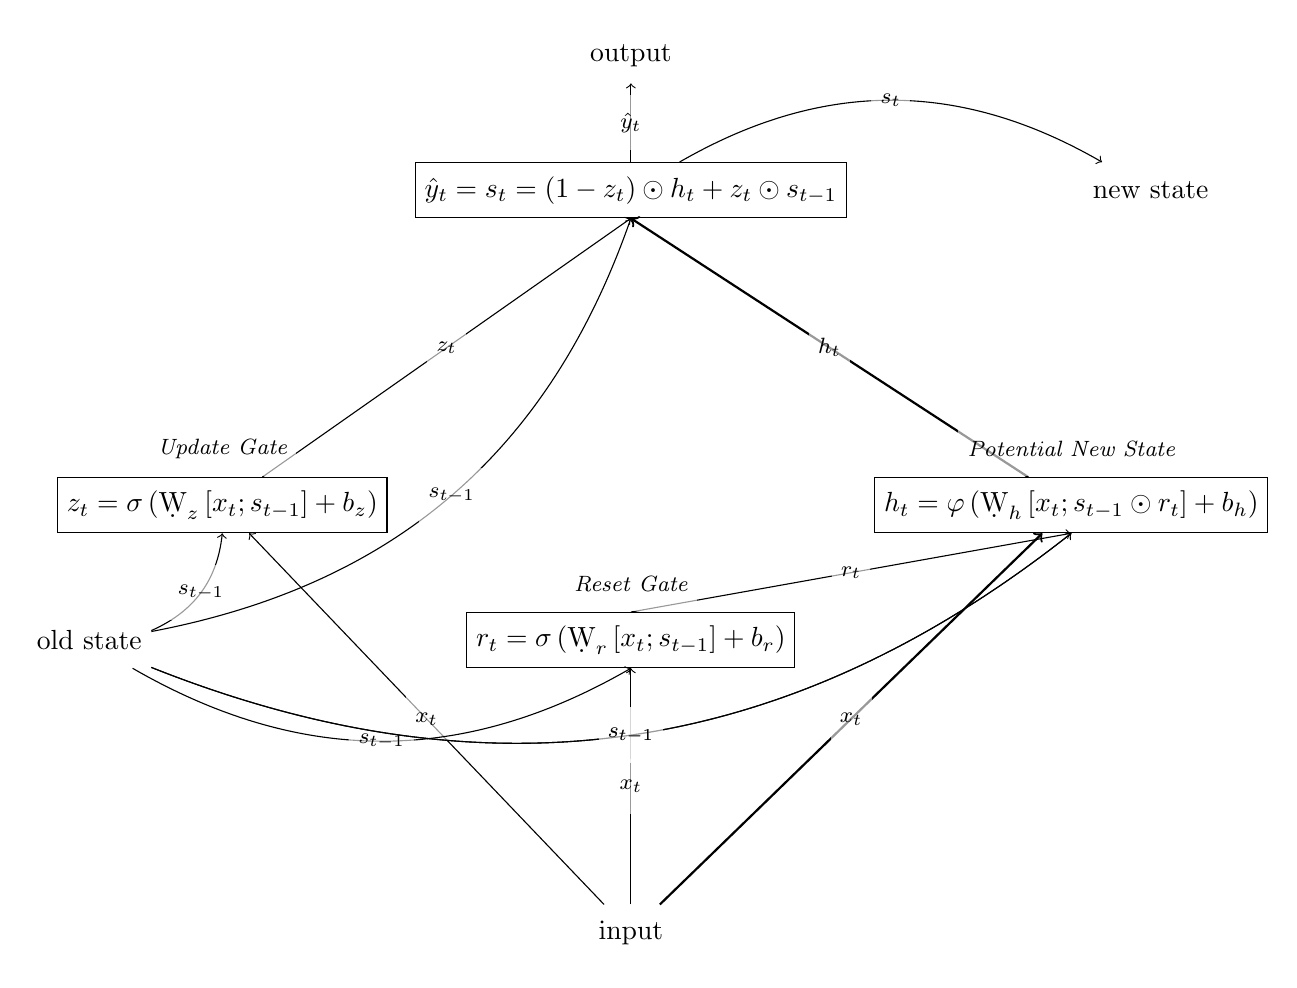
\begin{tikzpicture}[]
		\node(hidden)[layer]{$\nv h_t = \varphi \left( \d W_h\left[\nv x_t; \nv s_{t-1} \odot \nv r_t\right] + \dv b_h \right) $};
		\node(reset)[layer, below left=of hidden]{$\nv r_t = \sigma \left( \d W_r \left[\nv x_t; \nv s_{t-1}\right] + \dv b_r \right) $};
		\node(update)[layer, above left=of reset]{$\nv z_t = \sigma \left( \d W_z \left[\nv x_t; \nv s_{t-1}\right] + \dv b_z \right)$};
		\node(state)[layer, above = 5 of reset]{$\n \hat{y}_t=\nv s_t = (1-\nv z_t) \odot \nv h_t + \nv z_t \odot \nv s_{t-1}$};
		
		\node(in)[below = 3 of reset]{input};
		\node(stm)[left = 4 of reset]{old state};
		\node(stp)[right = 3 of state]{new state};
		\node(out)[above = of state]{output};
		
		\draw[->] (in) edge node[labe] {$\nv x_t$} (update);	
		\draw[->, bend right] (stm) edge node[labe] {$\nv s_{t-1}$} (update.south);
		\draw[->] (in) edge node[labe] {$\nv x_t$} (reset);	
		\draw[->, bend right] (stm) edge node[labe] {$\nv s_{t-1}$} (reset.south);
		
		\draw[->, thick] (in) edge node[labe] {$\nv x_t$} (hidden);	
		\draw[->, bend right] (stm) edge node[labe] {$\nv s_{t-1}$} (hidden.south);		
		\path[->] (reset.north) edge node[labe] {$\nv r_t$} (hidden.south);
		\draw[->, bend right] (stm) edge node[labe] {$\nv s_{t-1}$} (hidden.south);
		
		\draw[->, bend right] (stm) edge node[labe] {$\nv s_{t-1}$} (state.south);
		\draw[->, thick] (hidden) edge node[labe] {$\nv h_t$} (state.south);
		\draw[->] (update) edge node[labe] {$\nv z_t$} (state.south);
		\draw[->, bend left] (state) edge node[labe] {$\nv s_t$} (stp);
		\draw[->] (state) edge node[labe] {$\n \hat{y}_t$} (out);
		
		\node(updatelbl)[labe, above= 0 of update]{Update Gate};
		\node(resetlbl)[labe, above= 0 of reset]{Reset Gate};
		\node(hiddenlbl)[labe, above= 0 of hidden]{Potential New State};
		\end{tikzpicture}
	\end{adjustbox}
\end{figure}


The gated recurrent unit (GRU) is defined by:
\begin{align}
\nv z_t &= \sigma \left( \d W_z \left[\nv x_t; \nv s_{t-1}\right] + \dv b_z \right) \\
\nv r_t &= \sigma \left( \d W_r \left[\nv x_t; \nv s_{t-1}\right] + \dv b_r \right) \\
%
\nv h_t &= \varphi \left( \d W_h\left[\nv x_t; \nv s_{t-1} \odot \nv r_t\right] + \dv b_h \right)  \label{equ:gru-hidden}\\
\nv s_t &= (1-\nv z_t) \odot \nv h_t + \nv z_t\odot \nv s_{t-1} \label{equ:gru-state}\\
\n \hat{y}_t &= \nv s_t \label{equ:gru-outstate}
\end{align}
where $\d W_z$,$\d W_r$ and $\d W_h$ are the weight-vectors, and $\dv b_z$, $\dv b_r$ and $\dv b_h$are the bias vectors for the 3 separate layers.

\aside[Trade-off formula]{It may be stating the obvious, 
	but a standard way (and the only sensible way) to trade-off a value between two possible choices: $a$ and $b$,
	when given a preference level for the first as $p$ (a number between zero and one) is $(p)a+(1-p)b$.
	If $p$ is interpreted as the probability of $a$ being the correct value of a random variable, with $b$ as the other possible value, then this is the expected value of that random variable.}

This may look complex, but it can be broken down into parts.
First we can see that, like in the basic RU, the output and the state have the same value (\Cref{equ:gru-outstate}).

The $\nv h_t$  (\Cref{equ:gru-hidden}) is our core layer, as in the basic cell.
However, unlike in the basic cell, it does not immediately become the state: $\nv s_t$.
There is a trade-off (\Cref{equ:gru-state}) between the state keeping its old value $\nv s_{t-1}$, and getting the hidden layer value $\nv h_t$.
This trade-off is element-wise controlled by $\nv z_t$ which is valued between 0 and 1 (due to the sigmoid unit).
When an element of $\nv z_t$ is $1$, then the value of $\nv s_{t-1}$ for the corresponding element is kept.
Conversely, when the $\nv z_t$ element is $0$,  then the element of the new state is fully given by $\nv h_t$.

The $\nv z_t$ is often called the \emph{update gate} as it controls (``gates'') how much the state is updated using the new value in $\nv h_t$.
The update-gate sub-network uses the previous state $\nv s_{t-1}$ and the present input $\nv x_t$ to make this determination.

\aside[Multiplication, Concatenation, \\and Addition]{
	It is important to grasp that the product of a matrix and the concentration of two vectors can also be expressed as the sum of the product of a block of that matrix.
	They are the same thing.
	
	\mbox{$W\cdot \left[\v a; \v b\right] = U\v a + V \v b$}
	if  \mbox{$W=[U\; V]$}
		
	The difference is purely notation.
}

The \emph{reset gate} is loosely similar to the update gate.
$\nv r_t$ controls how much influence the past state $\nv s_{t-1}$ has on calculating the new value of $\nv h_t$ -- which is the new potential state/output as discussed.
It is perhaps clearer if $\nv h_t$ is reformulated to split $V$ into the terms which multiply with $\nv x_t$ and the terms which multiply with $\nv s_{t-1}$.

For $\d W_h = \left[\d W_{hx}\; \d W_{hs} \right]$ we can write:
\begin{align}
\nv h_t &= \varphi \left( \d W_h\left[\nv x_t; \nv s_{t-1} \odot \nv r_t\right] + \dv b_h \right)  \\
&= \varphi \left( \d W_{hx} \nv x_t + \d W_{hs} \left( \nv s_{t-1} \odot \nv r_t \right) + \dv b_h \right)
\end{align}
%
The $\nv r_t$ is called the reset-gate because it wipes the effect of the old-state in calculating the potential new state $\nv h_t$.
When $\nv r_t$ is reduced to zero, then the updated value for $\nv h_t$ is as if $\nv s_{t-1}$ was just like for the initial zero-vector state -- it is zeroed out by $\nv r_t$.
If the update gate $\nv z_t$ is high then it would fully reset the system.


Notice that when $\nv z_t=0$ and $\nv r_t=1$, then the system is identical to the Basic RU.
This could be achieved by setting suitably large biases.
However, the system is more flexible than that, 
since $\nv z_t$ and $\nv r_t$ are themselves very similar to Basic RUs -- though they do not control their own state.
The gates can behave differently based on the inputs and states to recognise the most important information that must be stored.



\subsection{LSTM Recurrent Unit}\label{sec:ltsm}
The LSTM is the most well known RNN unit.
The term is very nearly interchangeable with RNN today.
The original form was proposed by \tcite{hochreiter1997long}.
The form in current use is a variant from \tcite{gers1999learning}.

LSTM uses a compound state, comprised of the units previous output, and an additional state vector called the \emph{cell}.
We write $\nv s_t = (\nv c_t, \n \hat{y}_t)$,
to fit the normal formulation,
though for maths it is easier to work with these in parts.

\aside[Biasing the Forget Gate]{
	Practically, it is important to initially set the forget gate bias to 1.
	This is unlike all the other initialisation in the networks to 0 (or a small random number e.g. \texttt{randn(0.01)}).
	Equivalently one can also just add a constant additional bias term of ${+}1$ to the forget gate equations.
	This has been show to benefit almost all uses of LSTM \parencite{gers1999learning,jozefowicz2015empirical}.
	This is the default in most neural network libraries (though only recently patched in some).
}

\begin{align}
\nv s_t &= (\nv c_t, \n \hat{y}_t)\\
%
\nv i_t &= \sigma \left( \d W_i \left[\nv x_t; \hat{y}_{t-1}\right] + \dv b_i \right) \\
\nv f_t &= \sigma \left( \d W_f\left[\nv x_t; \hat{y}_{t-1}\right] + \dv b_f \right) \\
\nv o_t &= \sigma \left( \d W_o\left[\nv x_t; \hat{y}_{t-1}\right] + \dv b_o \right) \\
%
\nv h_t &= \tanh \left( \d W_h\left[\nv x_t; \hat{y}_{t-1}\right] + \dv b_h \right) \\
\nv c_t &=  \nv i_t\odot \nv h_t + \nv f_t \odot \nv c_{t-1} \\
\n \hat{y}_t &= \nv o_t \odot \varphi(\nv c_t)
\end{align}



In LSTM there are three gate sub-networks:
the input gate $\nv i_t$, the forget gate $\nv f_t$, and the output gate $\nv o_t$.

Together the input and forget-gates take the purpose of the GRU's update-gate.
Consider the case if $\nv o_t=1$ and $\varphi$ is the identify function,
and with $\nv i_t=1-\nv f_t$, that would make the value for $\nv c_t$ very similar to GRU's $\nv s_t$ (and $\n \hat{y}_t$ identical).


Individually, the forget gate $\nv f_t$ controls the extent that the previous value of the cell is used,
and the input gate $\nv i_t$ controls the extent to which the new potential value $\nv h_t$ is used for the new value of $\nv c_t$.

The output-gate's obvious purpose is to gate the output $y_t$.
However, as the output forms part of the state,
this has an effect on the networks next time-step.
Loosely this can be seen as similar to the GRU's reset gate.
If we substitute the value for $\hat{y}_{t-1} = \nv o_{t-1} \odot \varphi(\nv c_{t-1})$
into $\nv h_t$:
\begin{align}
\nv h_t &= \tanh \left( \d W_h\left[\nv x_t; \hat{y}_{t-1}\right] + \dv b_h \right) \\
\nv h_t &= \tanh \left( \d W_h\left[\nv x_t;  \nv o_{t-1} \odot \varphi(\nv c_{t-1})\right] + \dv b_h \right) 
\end{align}
it can be seen that, at the previous time-step, setting an element of $o_{t-1}$ to zero effectively removes the effect of the previous cell-state from the equations for all the gates and the the potential new cell $\nv h_t$.
Thus resetting the network.
(Similar substitutions can be done for $\nv i_t$, $\nv f_t$ and $\nv o_t$)


\begin{figure}
	\caption{A LSTM Recurrent unit.}
	\label{fig:lstm}
	\begin{adjustbox}{max width=\textwidth}
		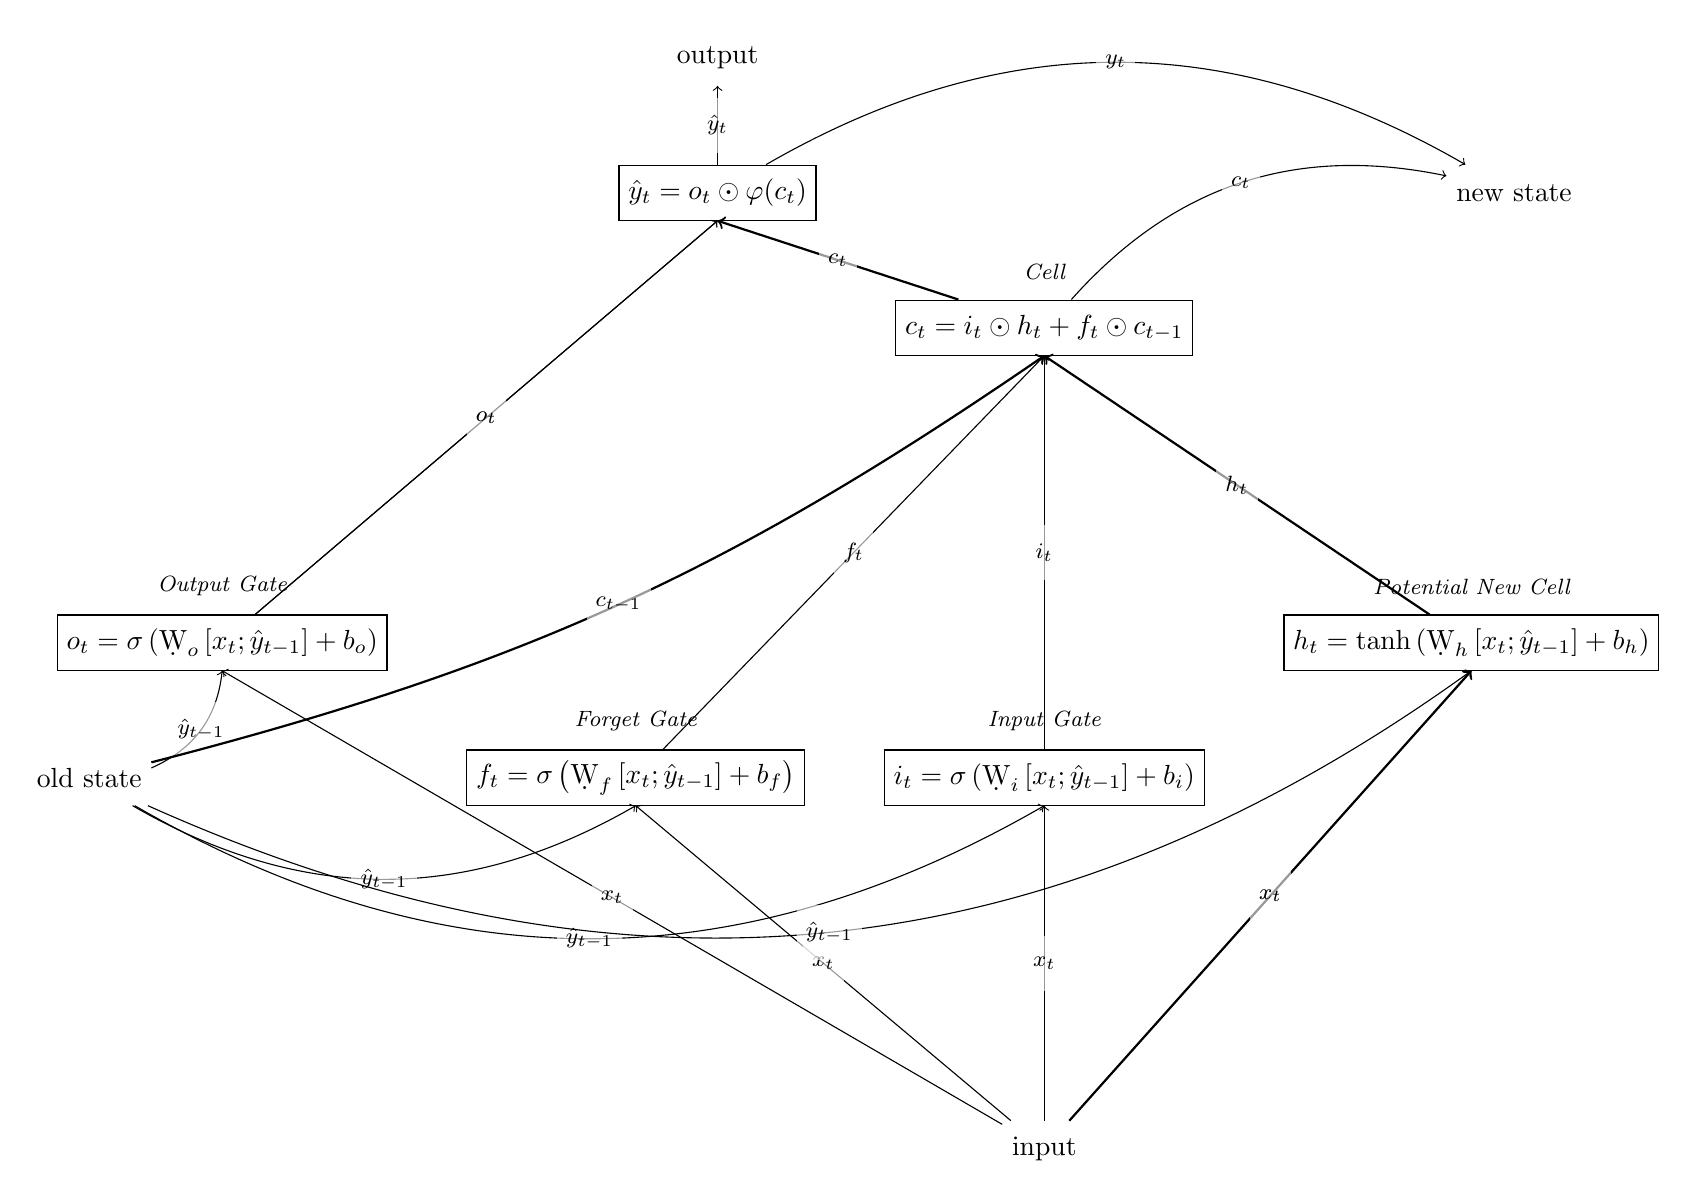
\begin{tikzpicture}[]
		\node(hidden)[layer]{$\nv h_t = \tanh \left( \d W_h\left[\nv x_t; \hat{y}_{t-1}\right] + \dv b_h \right)$};
		\node(igate)[layer, below left=of hidden]{$\nv i_t = \sigma \left( \d W_i \left[\nv x_t; \hat{y}_{t-1}\right] + \dv b_i \right)$};
		\node(fgate)[layer, left=of igate]{$\nv f_t = \sigma \left( \d W_f\left[\nv x_t; \hat{y}_{t-1}\right] + \dv b_f \right)$};
		\node(ogate)[layer, above left=of fgate]{$\nv o_t = \sigma \left( \d W_o\left[\nv x_t; \hat{y}_{t-1}\right] + \dv b_o \right)$};
		\node(state)[layer, above = 5 of igate]{$\nv c_t =  \nv i_t\odot \nv h_t + \nv f_t \odot \nv c_{t-1}$};
		\node(preout)[layer, above left = of state]{$\n \hat{y}_t = \nv o_t \odot \varphi(\nv c_t)$};
		
		\node(in)[below = 4 of igate]{input};
		\node(stm)[left = 4 of fgate]{old state};
		\node(stp)[right = 8 of preout]{new state};
		\node(out)[above = of preout]{output};
		
		
		\node(flbl)[labe, above= 0 of fgate]{Forget Gate};
		\node(ilbl)[labe, above= 0 of igate]{Input Gate};
		\node(olbl)[labe, above= 0 of ogate]{Output Gate};
		\node(hiddenlbl)[labe, above= 0 of hidden]{Potential New Cell};
		\node(statelbl)[labe, above= 0 of state]{Cell};
		
		\foreach \gate in {fgate, igate, ogate, hidden}{
			\draw[->, bend right] (stm) edge node[labe] {$\hat{y}_{t-1}$} (\gate.south);
			\draw[->] (in) edge node[labe] {$x_{t}$} (\gate.south);
		};
		\draw[->, bend right=10, thick] (stm) edge node[labe] {$c_{t-1}$} (state.south);
		
		\draw[->, thick] (in) edge node[labe] {$x_{t}$} (hidden.south);
		
		
		\draw[->] (fgate) edge node[labe] {$f_{t}$} (state.south);
		\draw[->] (igate) edge node[labe] {$i_{t}$} (state.south);
		\draw[->, thick] (hidden) edge node[labe] {$\nv h_t$} (state.south);
		
		
		
		\draw[->] (ogate) edge node[labe] {$o_{t}$} (preout.south);
		\draw[->] (ogate) edge node[labe] {$o_{t}$} (preout.south);
		
		\draw[->] (preout) edge node[labe] {$\hat{y}_{t}$} (out.south);
		
		\draw[->, thick] (state) edge node[labe] {$c_{t}$} (preout.south);
		
		\draw[->, bend left] (state) edge node[labe] {$c_{t}$} (stp);
		\draw[->, bend left] (preout) edge node[labe] {$y_{t}$} (stp);
		
		
		
		\end{tikzpicture}
	\end{adjustbox}
\end{figure}

\section{Further Variants}
\subsection{Deep Variants}
One can have a deep RNN.
This is done by stacking additional recurrent units above the existing ones.
Attaching, the unit output as the unit input of the layer above.
The result can be interpreted as a single, deep recurrent unit.

\subsection{Bidirectional RNNs}\label{sec:bidirection-rnns}
A Bidirectional RNN is similar to deep variants \pcite{schuster1997bidirectional}.
This is effectively using two RNNs so that the input can be processed from both temporal directions.
The forwards and backwards RNNs both take the same input at each time-step, but are otherwise fully distinct.
The unit outputs at each time-step are concatenated to give an overall time-step output from the RUs.

This is not so useful in most decoder RNNs, the number of outputs (and thus time-steps) of a decoder RNN is not known except by running them until an end-marker is output.
However, there are absolutely no issues when using them for an encoder.
In an encoder network the whole input is available before the output needs to be produced.
Similarly for a matched-sequence RNN, if  the sequence can be broken down into blocks (e.g. sentences), and a real-time output is not required


\subsection{Other RNNs}
There also exist many other RNNs.
Some are similar in structure to those discussed and can be analysed similarly via their recurrent units.
Such as the two models of \tcite{mikolovLongerSTM}, which incorporate a decaying sum of past states into the current state (either gated, or constant).
Other networks incorporate various other data-structures (or analogies to such structures) into their recurrent structure:
such as stacks \pcite{stacklstm}, pointers/arrays \pcite{MemoryNN}, or tapes \pcite{DBLP:journals/corr/GravesWD14}.

As natural language is primarily a sequential task, RNNs in various forms will be discussed in almost every chapter of this book.

\printbib

\end{document}